\part{Quantum Physics}
\section{}

The photoelectric effect implies that light has particle nature. When a light is shon on a photo emmitter it causes electrons to be emitted following the following equation:
\[eV_s=hf-\varphi\]
Where \(e\) is the charge of an electron, \(V_s\) is the stopping voltage required to stop current flow, \(h\) is plank's constant \(h=\num{6.626e-34}\), \(f\) is the frequency of the incident light and \(\varphi\) is the workfunction which is the value \(hf_0\) such that \(hf-hf_0=0\) where \(f_0\) is the minimum frequency.

When shone on a slit electrons will diffract, this shows that they have wave like nature.

\subsection*{Wave function}

The wave function \(\psi\) is a multivariable function \(\psi(x,y,z,t)\) where \(x,y\) and \(z\) are the three spatial dimensions and \(t\) is time. For this course we will only look at one dimensional functions which are time independent (time doesn't effect the potential energy of the particle). These take the form \(\psi(x)\). An example would be \(\psi_+\):
\[\psi_+(x)=Ae^{ikx}\]
where \(A\) and \(k\) are constants. There is another solution closely linked to this one and also both can be written in a different form:
\[\psi_+(x)=Ae^{ikx}=A(\cos kx+i\sin kx)\qquad\psi_-(x)=Ae^{-ikx}=A(\cos kx-i\sin kx)\]
These are waves. It is possible to work out the probability of the wave being found in a particular space using the probability function \(|\psi|^2=\psi\cc\psi\). For the example \(\psi=Ae^{ikx}\):
\[\psi=Ae^{ikx}\implies\cc\psi=Ae^{-ikx}\]
\[|\psi|^2=\psi\cc\psi=Ae^{ikx}Ae^{-ikx}=A^2e^{ikx-ikx}=A^2\]
This is independent of \(x\) and therefore the particle is equally likely to be at any point in space.

\subsection*{The Schr\"odinger equation}

\begin{center}
\boxed{\dv[2]{\psi}{x}+\frac{8\pi^2m}{h^2}[E-U(x)]\psi=0}
\end{center}

In this equation \(m\) is the mass of the particle, \(E\) is the total energy of the system and \(U(x)\) is the potential energy of the system. For the case where \(U(x)\) is independent of \(x\) since the point at which \(U(x)=0\) is arbitrary we can just set it equal to 0 so we get:
\[\dv[2]{\psi}{x}+\frac{8\pi^2m}{h^2}E\psi=0\]

It is possible to show that our example from before satisfies the equation under certain conditions:
\begin{align*}
\psi&=Ae^{ikx}\\
\dv{\psi}{x}&=Aike^{ikx}\\
\dv[2]{\psi}{x}&=-Ak^2e^{ikx}
\end{align*}

Substituting into the Schr\"odinger equation:
\[-Ak^2e^{ikx}+\frac{8\pi^2m}{h^2}EAe^{ikx}=0\]
\[-k^2+\frac{8\pi^2m}{h^2}E=0\]
So \(\psi=Ae^{ikx}\) is a solution if:
\[E=\frac{h^2k^2}{8\pi^2m}\iff k^2=\frac{8\pi^2mE}{h^2}\]

The reduced plank's constant \(\hb\) is defined as \(\hb\triangleq\frac{h}{2\pi}\). Using this we can write the conditions as:
\[E=\frac{\hb^2k^2}{2m}\iff k^2=\frac{mE}{\hb^2}\]
Note that this only applies for a free particle (a particle with a boundary will have \(U(x)\) that depends on \(x\)). The whole Schr\"odinger equation can be written as:
\[\dv[2]{\psi}{x}+\frac{2m}{\hb^2}[E-U(x)]\psi=0\]


\section{}

Using \(\hb\) we get \(E=\hb\omega\)

From last lecture we saw that if \(\psi_+=Ae^{ikx}\) is a solution then \(k^2=\frac{8\pi^2m}{h^2}E\) If this is true then the Schr\"odinger equation can be rewritten as:
\[\dv[2]{\psi}{x}+k^2\psi=0\]
This is the wave equation.

\(k\) is the wave number in this equation. It is the number of waves per unit distance.

\[k^2=\frac{8\pi^2m}{h^2}E\implies E=\frac{k^2h^2}{8\pi^2m}\]
For non relativistic particles \(E=\frac{p^2}{2m}=\frac{m^2v^2}{2m}=\frac12mv^2\)
\[E=\frac{h^2k^2}{8\pi^2m}=\frac{p^2}{2m}\]
\[p^2=\frac{h^2k^2}{4\pi^2}\]
\[p=\frac{hk}{4\pi^2}=\hb k\]
The momentum \(p\) of a solution to the free Scr\"odinger equation is given by \(p=\hb k\)

A more realistic solution to the Schr\"odinger equation is the sum of sinusoidal terms of different frequencies:
\[\psi(x)=\sum_jAe^{ik_jx}\]

\begin{tikzpicture}[scale=0.75]
\begin{axis}[
    title={\(\psi_1\)},
    axis lines = left,
    axis lines = center,
    xtick style={draw=none},
    ytick style={draw=none},
    xticklabels={},
    yticklabels={},
    xlabel = {},
    ylabel = {},
]

\addplot [
    domain=0:12.566, 
    samples=100, 
    color=black,
]
{sin(deg(x))};
 
\end{axis}
\end{tikzpicture}
\begin{tikzpicture}[scale=0.75]
\begin{axis}[
    title={\(\psi_2\)},
    axis lines = left,
    axis lines = center,
    xtick style={draw=none},
    ytick style={draw=none},
    xticklabels={},
    yticklabels={},
    xlabel = {},
    ylabel = {},
]

\addplot [
    domain=0:12.566, 
    samples=100, 
    color=black,
]
{sin(deg(0.95*x))};
 
\end{axis}
\end{tikzpicture}
\begin{tikzpicture}[scale=0.75]
\begin{axis}[
    title={\(\psi_3\)},
    axis lines = left,
    axis lines = center,
    xtick style={draw=none},
    ytick style={draw=none},
    xticklabels={},
    yticklabels={},
    xlabel = {},
    ylabel = {},
]

\addplot [
    domain=0:12.566, 
    samples=100, 
    color=black,
]
{sin(deg(0.9*x))};
 
\end{axis}
\end{tikzpicture}
\begin{tikzpicture}[scale=0.75]
\begin{axis}[
    title={\(\psi_4\)},
    axis lines = left,
    axis lines = center,
    xtick style={draw=none},
    ytick style={draw=none},
    xticklabels={},
    yticklabels={},
    xlabel = {},
    ylabel = {},
]

\addplot [
    domain=0:12.566, 
    samples=100, 
    color=black,
]
{sin(deg(0.85*x))};
 
\end{axis}
\end{tikzpicture}
\begin{tikzpicture}[scale=0.75]
\begin{axis}[
    title={\(\psi_5\)},
    axis lines = left,
    axis lines = center,
    xtick style={draw=none},
    ytick style={draw=none},
    xticklabels={},
    yticklabels={},
    xlabel = {},
    ylabel = {},
]

\addplot [
    domain=0:12.566, 
    samples=100, 
    color=black,
]
{sin(deg(0.8*x))};
 
\end{axis}
\end{tikzpicture}
\begin{tikzpicture}[scale=0.75]
\begin{axis}[
    title={\(\psi_6\)},
    axis lines = left,
    axis lines = center,
    xtick style={draw=none},
    ytick style={draw=none},
    xticklabels={},
    yticklabels={},
    xlabel = {},
    ylabel = {},
]

\addplot [
    domain=0:12.566, 
    samples=100, 
    color=black,
]
{sin(deg(0.75*x))};
 
\end{axis}
\end{tikzpicture}
\begin{tikzpicture}[scale=0.75]
\begin{axis}[
    title={\(\psi_7\)},
    axis lines = left,
    axis lines = center,
    xtick style={draw=none},
    ytick style={draw=none},
    xticklabels={},
    yticklabels={},
    xlabel = {},
    ylabel = {},
]

\addplot [
    domain=0:12.566, 
    samples=100, 
    color=black,
]
{sin(deg(0.7*x))};
 
\end{axis}
\end{tikzpicture}
\begin{tikzpicture}[scale=0.75]
\begin{axis}[
    title={\(\psi_8\)},
    axis lines = left,
    axis lines = center,
    xtick style={draw=none},
    ytick style={draw=none},
    xticklabels={},
    yticklabels={},
    xlabel = {},
    ylabel = {},
]

\addplot [
    domain=0:12.566, 
    samples=100, 
    color=black,
]
{sin(deg(0.65*x))};
 
\end{axis}
\end{tikzpicture}
\begin{tikzpicture}[scale=0.75]
\begin{axis}[
    title={\(\psi_9\)},
    axis lines = left,
    axis lines = center,
    xtick style={draw=none},
    ytick style={draw=none},
    xticklabels={},
    yticklabels={},
    xlabel = {},
    ylabel = {},
]

\addplot [
    domain=0:12.566, 
    samples=100, 
    color=black,
]
{sin(deg(0.6*x))};
 
\end{axis}
\end{tikzpicture}
\begin{tikzpicture}[scale=0.75]
\begin{axis}[
    title={\(\psi_{10}\)},
    axis lines = left,
    axis lines = center,
    xtick style={draw=none},
    ytick style={draw=none},
    xticklabels={},
    yticklabels={},
    xlabel = {},
    ylabel = {},
]

\addplot [
    domain=0:12.566, 
    samples=100, 
    color=black,
]
{sin(deg(0.55*x))};
 
\end{axis}
\end{tikzpicture}
\begin{tikzpicture}[scale=0.75]
\begin{axis}[
    title={\(\psi_{11}\)},
    axis lines = left,
    axis lines = center,
    xtick style={draw=none},
    ytick style={draw=none},
    xticklabels={},
    yticklabels={},
    xlabel = {},
    ylabel = {},
]

\addplot [
    domain=0:12.566, 
    samples=100, 
    color=black,
]
{sin(deg(0.5*x))};
 
\end{axis}
\end{tikzpicture}
\begin{tikzpicture}[scale=0.75]
\begin{axis}[
    title={\(\psi_{12}\)},
    axis lines = left,
    axis lines = center,
    xtick style={draw=none},
    ytick style={draw=none},
    xticklabels={},
    yticklabels={},
    xlabel = {},
    ylabel = {},
]

\addplot [
    domain=0:12.566, 
    samples=100, 
    color=black,
]
{sin(deg(0.45*x))};
 
\end{axis}
\end{tikzpicture}
\begin{center}
\begin{tikzpicture}[scale=1]
\begin{axis}[
    title={\(\sum_{j=1}^{12}\psi_j\)},
    axis lines = left,
    axis lines = center,
    xtick style={draw=none},
    ytick style={draw=none},
    xticklabels={},
    yticklabels={},
    xlabel = {},
    ylabel = {},
]

\addplot [
    domain=-15.708:15.708, 
    samples=100, 
    color=black,
]
{sin(deg(0.95*x))+sin(deg(0.9*x))+sin(deg(0.85*x))+sin(deg(0.8*x))+sin(deg(0.75*x))+sin(deg(0.7*x))+sin(deg(0.65*x))+sin(deg(0.6*x))+sin(deg(0.55*x))+sin(deg(0.5*x))+sin(deg(0.45*x))};
 
\end{axis}
\end{tikzpicture}
\end{center}

This superposition of different wave frequencies is known as a wave packet. The wave packet is also a solution to the Schr\"odinger equation. The particle isn't equally likely to be anywhere, it is now localised.

Each frequency has an associated wave number \(k_j\). The momentum is \(p=\hb k\) so the momentum is now no longer known precisely. We have an uncertainty of \(\Delta p\). The smaller the wave packet the more localised the particle is and the greater the range of frequencies needed. This gives rise to Heisenberg's uncertainty principle:
\[\Delta x\Delta p_x\ge\frac\hb2\]
Where \(\Delta x\) is uncertainty in position and \(\Delta p_x\) is uncertainty in momentum in the \(x\) direction. This fundamentally limits how well we can measure \(p_x\) and \(x\). A similar relationship between energy and time exists:
\[\Delta E\Delta t\ge\frac\hb2\]

\section{}

If we introduce a potential \(U(x)\) then only certain energies \(E\) are allowed. The energy becomes quantised.

\(\psi_+(x)=Ae^{ikx}\) is a particle moving in the positive \(x\) direction. \(\psi_-(x)=Ae^{-ikx}\) is a particle moving in the negative \(x\) direction. If we sum them together we get a standing wave:
\[\psi=\psi_++\psi_-=Ae^{ikx}+Ae^{-ikx}=A[\cos kx+i\sin kx+\cos kx-i\sin kx]=2A\cos kx\]

A more general solution to the wave equation is given by \(\psi_+=Ae^{i(kx+\varphi)}\):
\[\diff x (Ae^{i(kx+\varphi)})=Aike^{i(kx+\varphi)}\]
\[\diff[2] x(Ae^{i(kx+\varphi)})=-Ak^2e^{i(kx+\varphi)}\]
\[-Ak^2e^{i(kx+\varphi)}+\frac{8\pi^2m}{h^2}[E-u(x)]Ae^{i(kx+\varphi)}=0\]
So given the condition \(k^2=\frac{8\pi^2m}{h^2}\) this is a solution.
The standing wave formed with this solution is:
\[\psi=\psi_++\psi_-=2A\cos(kx+\varphi)=2A\sin\left(kx+\varphi-\frac{\pi}{2}\right)\]
This shows that the standing waves which satisfy the Schr\"odinger equation are sinusoidal.

\subsection*{Infinite square potential}

\begin{center}
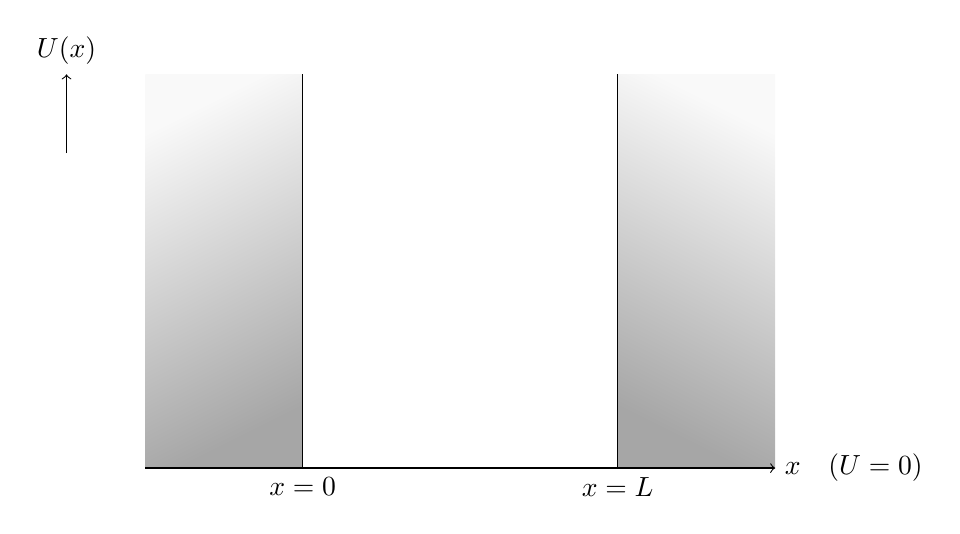
\begin{tikzpicture}
\shade [left color=gray!5, right color=gray!70, shading=axis, shading angle=26.565] (-2,0) -- (-4,0) -- (-4,5) -- (-2,5) -- (-2,0);
\shade [right color=gray!5, left color=gray!70, shading=axis, shading angle=153.435] (2,0) -- (4,0) -- (4,5) -- (2,5) -- (2,0);
\draw [->] (-4,0) -- (4,0);
\draw (-2,0) -- (-2,5);
\draw (2,0) -- (2,5);
\draw [->] (-5,4) -- (-5,5);
\node [below] at (-2,0) {\(x=0\)};
\node [below] at (2,0) {\(x=L\)};
\node [above] at (-5,5) {\(U(x)\)};
\node [right] at (4,0) {\(x\quad (U=0)\)};
\end{tikzpicture}
\end{center}
No particles can be at \(x\) values outside of the range \(x\in(0,L)\). This means that the probability density function (p.d.f.) is 0 outside of this range:
\[|\psi(0)|^2=|\psi(L)|^2=0\]
\[\implies\psi(0)=\psi(L)=0\]
A standing wave with nodes at \(x=0\) and \(x=L\) is therefore a valid solution to the Scr\"odinger equation in this case:

\begin{center}
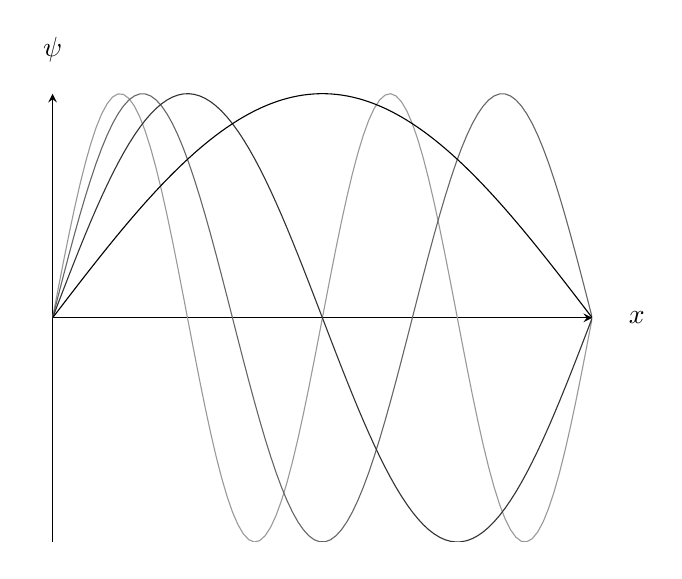
\begin{tikzpicture}[scale=1]
\begin{axis}[
    axis lines = left,
    axis lines = center,
    xtick style={draw=none},
    ytick style={draw=none},
    xticklabels={},
    yticklabels={},
    xlabel = {\(x\)},
    ylabel = {\(\psi\)},
every axis x label/.style={
    at={(ticklabel* cs:1.05)},
    anchor=west,
},
every axis y label/.style={
    at={(ticklabel* cs:1.05)},
    anchor=south,
},
]

\addplot [
    domain=0:3.1415926, 
    samples=100, 
    color=black!40,
]
{sin(deg(4*x))};

\addplot [
    domain=0:3.1415926, 
    samples=100, 
    color=black!60,
]
{sin(deg(3*x))};

\addplot [
    domain=0:3.1415926, 
    samples=100, 
    color=black!80,
]
{sin(deg(2*x))};

\addplot [
    domain=0:3.1415926, 
    samples=100, 
    color=black,
]
{sin(deg(x))};
\end{axis}
\end{tikzpicture}
\end{center}
The solution has wavelength \(\lambda\) which can take the values:
\[\lambda=2L,L,\frac 23L,\frac12L,\cdots\]
Since \(k=\frac{2\pi}{\lambda}\) then \(k\) can take the values:
\[k=\frac{\pi}{L},\frac{2\pi}{L},\frac{3\pi}{L},\frac{4\pi}{L},\cdots=\frac{n\pi}{L}\quad n\in\bb N\]
Here \(n\) is the quantum number \(n=1,2,3,4\cdots\)

In the region between \(x=0\) and \(x=L\) the particle is free so we can use:
\[E=\frac{\hb^2k^2}{2m}=\frac{\hb^2n^2\pi^2}{2mL^2}=\frac{h^2}{8mL^2}n^2\]

\begin{center}
\begin{tikzpicture}
\draw [->] (0,0) -- (0,5);
\node [above] at (0,5) {\(E\)};
\draw (0.5,0.5) -- (5,0.5);
\draw (0.5,2) -- (5,2);
\draw (0.5,4.5) -- (5,4.5);
\node [right] at (5,0.5) {\(\frac{h^2}{8mL^2}\)};
\node [right] at (5,2) {\(4\frac{h^2}{8mL^2}\)};
\node [right] at (5,4.5) {\(9\frac{h^2}{8mL^2}\)};
\end{tikzpicture}
\end{center}
The energy levels are getting further and further apart. Note that the lowest possible energy level is not 0 as \(n\ne0\)

\begin{center}
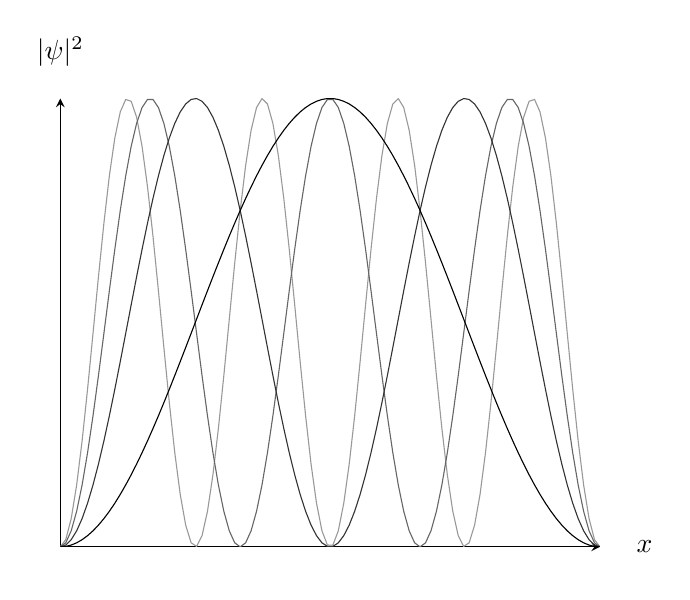
\begin{tikzpicture}[scale=1]
\begin{axis}[
    axis lines = left,
    axis lines = center,
    xtick style={draw=none},
    ytick style={draw=none},
    xticklabels={},
    yticklabels={},
    xlabel = {\(x\)},
    ylabel = {\(|\psi|^2\)},
every axis x label/.style={
    at={(ticklabel* cs:1.05)},
    anchor=west,
},
every axis y label/.style={
    at={(ticklabel* cs:1.05)},
    anchor=south,
},
]

\addplot [
    domain=0:3.1415926, 
    samples=100, 
    color=black!40,
]
{sin(deg(4*x))^2};

\addplot [
    domain=0:3.1415926, 
    samples=100, 
    color=black!60,
]
{sin(deg(3*x))^2};

\addplot [
    domain=0:3.1415926, 
    samples=100, 
    color=black!80,
]
{sin(deg(2*x))^2};

\addplot [
    domain=0:3.1415926, 
    samples=100, 
    color=black,
]
{sin(deg(x))^2};
\end{axis}
\end{tikzpicture}
\end{center}
This shows the p.d.f. for \(n=1,2,3,4\)

We can only measure the probability to find a particle in a region of width \(\Delta x\). To find if the particle is close to \(\frac L2\) we measure the probability to find the particle in \(x\in\left(\frac L2-\frac{\Delta x}{2},\frac L2 + \frac{\Delta x}{2}\right)\)
This means that for \(n=20\) we measure the red line when the p.d.f. looks like the black:

\begin{center}
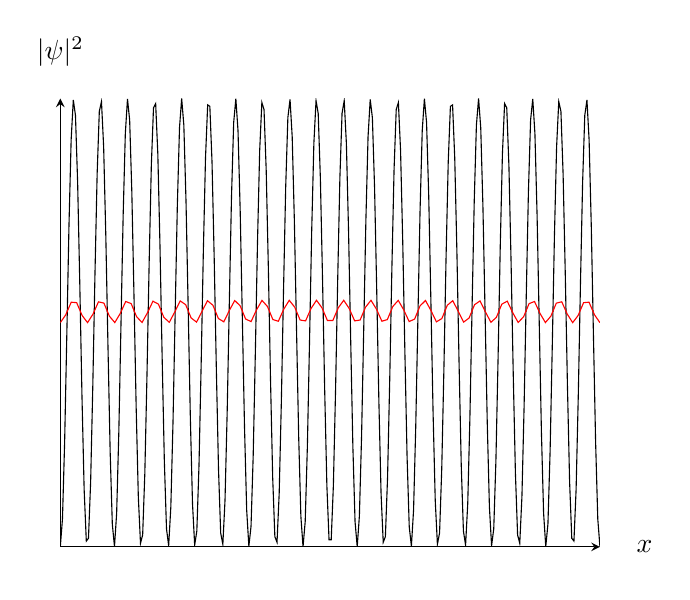
\begin{tikzpicture}
\begin{axis}[
    axis lines = left,
    axis lines = center,
    xtick style={draw=none},
    ytick style={draw=none},
    xticklabels={},
    yticklabels={},
    xlabel = {\(x\)},
    ylabel = {\(|\psi|^2\)},
every axis x label/.style={
    at={(ticklabel* cs:1.05)},
    anchor=west,
},
every axis y label/.style={
    at={(ticklabel* cs:1.05)},
    anchor=south,
},
]

\addplot [
    domain=0:3.1415926, 
    samples=250, 
    color=black,
]
{sin(20*deg(x))^2};

\addplot [
    domain=0:3.1415926, 
    samples=100, 
    color=red,
]
{(1/20)*sin(20*deg(x))^2+(1/2)};

\end{axis}
\end{tikzpicture}
\end{center}
This agrees better with what classical mechanics would predict. This is an example of the correspondence principle:

\begin{displayquote}
For sufficiently high quantum numbers the results predicted by quantum mechanics are indistinguishable from the results predicted by classical mechanics.
\end{displayquote}

This can be seen if we consider an air hockey puck on a air hockey table. This idealised system behaves as an infinite square potential. For a puck mass \(m=\SI{50}{g}\), velocity \(v=\SI{5}{m.s^{-1}}\) and a table of length \(L=\SI{2}{m}\) the energy of the puck is given by:
\[E=\frac 12mv^2=\frac 120.05\cdot 5^2=\frac 58\]
\[E_n=\frac{h^2n^2}{8mL^2}\]
\[n=\sqrt{\frac{8mL^2E_n}{h^2}}\]
\[n=\num{1.5e33}\]
\(n\) is very big so quantum predictions will agree with classical predictions.

\section{}

The lowest allowed energy is called the zero-point energy
\[\dv[2]{\psi(x)}{x} + \frac{8\pi^2m}{h^2}[E-U(x)]\psi(x)=0\]

We will consider the potential energy function
\[U(x)=\left\{
\begin{array}{l l}
0 & \text{for } x<L\\
U_1 & \text{for } x\ge L
\end{array}
\right.\]
Where \(U_1>E\). A solution to this is \(\psi(x)=Be^{-\alpha x}\) for \(\alpha\in\bb R\)
\[\dv{\psi}{x}=-\alpha Be^{-\alpha x},\qquad \dv[2]{\psi}{x}=\alpha^2Be^{-\alpha x}\]
\[\alpha^2 B e^{-\alpha x}+\frac{8\pi^2m}{h^2}\underbrace{[E-U_1]}_{<0}Be^{-\alpha x}=0\]
\[\alpha^2 +\frac{8\pi^2m}{h^2}[E-U_1]=0\]
\[\alpha^2=\frac{8\pi^2m}{h^2}\underbrace{[U_1-E]}_{>0}\]
\[\alpha = \sqrt{\frac{8\pi^2m}{h^2}[U_1-E]}\]

So depending on the values of \(\alpha\) and \(x\) \(\psi\) is either increasing or decreasing exponentially in the region where \(x\ge L\). Classically the particle wouldn't be allowed in this region but in quantum mechanics it is allowed. In the region where \(U(x) = 0\) \(\psi\) is a standing wave caused by partial reflection at the boundary. In the region where \(U(x) = U_1\) \(\psi\) decays exponentially. Importantly:
\begin{itemize}
\item \(\psi\ne 0\) in the classical forbidden region
\item The wave function transitions smoothly at the boundary
\item \(\psi\to0\) as\(x\to\infty\)
\end{itemize}

\subsection*{Harmonic Potential well}

\(U(x)=\frac 12k_{\text{spr}}x^2\) where \(k_{\text{spr}}\) is the spring constant not the wave number.

We expect sinusoidal standing waves in the classically allowed region and \(\psi\to0\) as \(x\to\pm\infty\)

\(\displaystyle{E_n=\left(n+\frac 12\right)\hb \omega}\) where \(\displaystyle{\omega = \sqrt{\frac{k_{\text{spr}}}{m}}}\) and \(n=0,1,2\dots\)

zero-point energy \(\displaystyle{E_0=\frac 12\hb\omega}\)

This creates evenly spaced energy levels. Inside the classical boundaries \(\psi\) is a standing wave, outside it decays exponentially.

\subsection*{Quantum tunnelling}

If instead we consider a potential
\[U(x) = \left\{
\begin{array}{l l}
0 & \text{for } L_1>x\\
U_1 & \text{for } L_1\le x<L_2\\
0 & \text{for } L_2\le x
\end{array}
\right.\]
Before the increased potential \(\psi\) is a large amplitude standing wave, between \(L_1\) and \(L_2\) \(\psi\) decays exponentially and after \(L_2\) \(\psi\) is a small amplitude standing wave.

\section{}

\subsection*{The Bohr Model of H}

The Bohr model is based on four unjustified postulates:
\begin{itemize}
\item Electrons orbit the nucleus at a fixed radius due to the Coulomb force
\item The angular momentum of the electron is quantised \(l=n\hb\) where \(n=1,2,3,\dots\)
\item The electron doesn't radiate photons when it is in one of these orbits
\item Emission/absorption occurs due to transitions between these orbits
\end{itemize}
Potential energy of an electron in H:
\[PE=U(r)=\frac{q_1q_2}{4\pi\varepsilon_0}=-\frac{e^2}{4\pi\varepsilon_0}\]
Electrostatic and centripetal forces balance:
\[\frac{mv^2}{r}=\frac{e^2}{4\pi\varepsilon_0}\implies KE = \frac 12mv^2=\frac{e^2}{8\pi\varepsilon_0r}\]
Total energy:
\[E=KE+PE=-\frac{e^2}{8\pi\varepsilon_0r}\tag{17.1}\]
The total energy is negative as the electron is bound to the atom and needs to gain energy to leave. Note that \(E\propto\frac 1r\)
\[l=mvr=n\hb\qquad n=1,2,3,\dots\tag{17.2}\]
Balancing forces:
\[\frac{mv^2}{r}=\frac{e^2}{4\pi\varepsilon_0r^2}\tag{17.3}\]
Rearranging (17.1) gives
\[v=\frac{n\hb}{mr}\]
Substituting this into (17.3) gives
\[\frac mr\left(\frac{n\hb}{mr}\right)^2=\frac{e^2}{4\pi\varepsilon_0r^2}\]
\[r=\frac{4\pi\varepsilon_0\hb^2}{me^2}n^2=\underbrace{\frac{\varepsilon_0h^2}{\pi me^2}}_{\text{constant}}n^2\]
Note that \(r\propto n^2\)

The smallest possible radius occurs at \(n=1\):
\[r_1=\frac{\varepsilon_0h^2}{\pi me^2}=\SI{5.29e-11}{m}=a\]
\(a\) is the Bohr radius. If we substitute this into (17.1) we get
\[E=-\frac{m^2e^4}{8\varepsilon_0^2h^2n^2}=-\frac{13.6}{n^2}\mskip3mu\si{eV}\]

\subsection*{Quantum Model}

The Bohr model misses several predictions that the quantum model successfully makes. The quantum model comes from solving the 3D time invariant Schr\"odinger equation for \(\psi(x,y,z)\)
\[\pd[2]{\psi}{x}+\pd[2]{\psi}{y}+\pd[2]{\psi}{z}+\frac{8\pi^2m}{h^2}[E-U(x,y,z)]\psi=0\]
\[U(x,y,z)=-\frac{e^2}{4\pi\varepsilon_0r}\quad\text{where}\quad r=\sqrt{x^2+y^2+z^2}\]
Using spherical polar coordinates \((r,\vartheta,\varphi)\), as the system is spherically symmetrical, the solution can be written as a product of functions dependant on quantum numbers \(n,l\) and \(m_l\)
\[\psi(r,\vartheta,\varphi)=R_{n,l}(r)\Theta_{l,m_l}(\vartheta)\Phi_{m_l}(\varphi)\]
This gives
\[E_n=-\frac{m^2e^4}{8\varepsilon_0^2h^2n^2}=-\frac{13.6}{n^2}\mskip3mu\si{eV}\]

\section{}

\begin{center}
\includegraphics[scale = 0.2]{SphericalPolarCoordinates}
\end{center}


We have to apply boundary conditions for the 3D Schr\"odinger equation that \(\psi\to0\) as \(x,y,z\to\infty\)

\(n\) is the principal quantum number. It determines the energy and radial extent of the wave function.

\(n=1,2,3,\dots\) \(n\in\bb N\)

\(l\) is the orbital angular momentum quantum number. It determines the magnitude of angular momentum.

\(l=1,2,\dots,n-1\) \(l\in\bb N\) and \(l<n\)

\(m_l\) is the magnetic quantum number. It determines the direction of angular momentum.

\(m_l=-l,-l+1,\dots,0,\dots l-1,l\) \(m_l\in\bb Z\) and \(|m_l|\le l\)

Suppose that \(n=2\), this means that \(l\) can take two values, 0 or 1. When \(l=0\) \(m_l=1\), when \(l=1\) \(m_l=-1,0,1\).

The angular momentum is given by \(|\vv L|=\sqrt{l(l+1)}\hb\). For \(l=1\) this means the angular momentum is \(|\vv L|=\sqrt{2}\hb\). Using \(m_l\) we can measure the components of \(\vv L\) in a direction. By convention we measure it for the \(z\) direction \(L_z=m_l\hb\). This gives us possible angular momentums \(\vv L\) as shown in the diagram

\begin{center}
\includegraphics[scale=0.4]{ElectronAngularMomentum}
\end{center}
This shows some of the possible angular momentum vectors \(\vv L\) for \(n=2\). The vectors are all from the origin to some point on the three dotted circles which lie in the planes \(z=-\hb,\,z=0\) and \(z=\hb\). The radius of the sphere is \(\sqrt 2\hb\).

If we proceed to measure a different component of the angular momentum we no longer know the component in the previously measured direction.

For \(n=1\)
\[R_{n=1}(r)=\frac{1}{\sqrt\pi a^{\frac32}}e^{-\frac ra}\]
Where \(a=\num{5.3e-11}\) is the Bohr radius

For a randomly chosen point in space the probability of it being a given distance \(r\) from the origin is proportional to the surface area of the sphere radius \(r\) which is \(4\pi r^2\)

When using \(\psi(r)\) instead of \(\psi(x)\) the radial probability density is
\[P(r)=4\pi r^2|\psi(r)|^2\]
For \(n=1\)
\[P_{n=1}(r)=4\pi r^2[R_{n=1}(r)]^2=\frac{4}{a^3}r^2e^{-\frac{2r}{a}}\]

\begin{center}
\includegraphics[scale=0.4]{RadialProbabilityDistribution}
\end{center}
The most likely radial distance is \(a\).

This gives rise to the orbitals. Each orbital is denoted by \(n\) and a letter representing \(l\):

\begin{center}
\begin{tabular}{|c|cccccc|}\hline
\(l\) & 0 & 1 & 2 & 3 & 4 & 5\\\hline
letter& s & p & d & f & g & h\\\hline
\end{tabular}
\end{center}
For example 1s is \(n=1,\,l=0\) and 3d is \(n=3,\,l=2\)


\section{}

Electrons also have spin quantum numbers \(s\) and \(m_s\). Spin is predicted when relativity is added to quantum mechanics. The magnitude of total spin \(|\vv S|\) is given by
\[|\vv S|=\sqrt{s(s+1)}\hb\]
The component of spin in the \(z\) direction is given by
\[S_z=m_s\hb\]
For electrons \(s=\frac12\). \(m_2\in\{-s,-s+1,\dots ,s-1,s\}\) so for an electron \(m_s=\pm\frac12\). Electrons are described by the four quantum numbers \(n,l,m_l\) and \(m_s\).
\[|\vv S|=\sqrt{s(s+1)}\hb=\frac{\sqrt{3}}{2}\]
\[S_z=m_s\hb=\pm\frac12\hb\]
For hydrogen the Schr\"odinger equation can be solved exactly. For multi-electron systems all of the electrons repel each other. This means it isn't possible to solve the Schr\"odinger equation exactly, however, numerical solutions can be found. In multi-electron systems the electrons may have the same quantum numbers as a single electron system but the energies will be different. In a multi-electron system the energy depends mostly on \(n\) and \(l\).

The Pauli exclusion principal states

\begin{displayquote}
No two fermions in a system may have the same quantum state
\end{displayquote}

A fermion is any particle with \(s=\frac{2m+1}{2}\) for \(m\in\bb Z\). This includes electrons, protons, neutrons, muons and neutrinos. Particles with \(s=m\) for \(m\in\bb Z\). This includes photons, the Higg's boson and \(^2\)He.

Spin up is used to refer to \(s=\frac12\) and spin down refers to \(s=-\frac12\).

A consequence of the Pauli exclusion principal is that each orbital can hold two electrons for each value of \(l\) (spin up and spin down). This means that each s orbital can hold two electrons, p orbitals can hold 6 , d orbitals can hold 10 and f orbitals can hold 14.

The probability per unit time of a transition between energy levels is not the same for all transitions. If \(\Delta l=1\) the transition is likely to occur and is said to be an allowed transition. If an electron can de-excite by such a transition it will and quickly. If \(\Delta l\ne 1\) then the transition is less likely and is said to be ``forbidden'' (but can still occur). If there are no other transitions possible an electron will de-excite by this transition but it will take a long time.

Flourescence is emission of light during illumination as the light excites electrons which then fall back to the ground state in several lower frequency stages emitting multiple photon along the way.

Phosphorecence is emission of light after illumination as the light excites electrons into forbiden transitions which then don't fall back to ground state for a long time, possibly after the illumination has been removed.

\section{}

Fast (allowed) transitions have small \(\Delta t\) and therefore large error in their energy \(\Delta E\).

Slow (forbidden) transitions have large \(\Delta t\) and therefore small error in their energy \(\Delta E\).

\(hf=E_1-E_2\) has some variance since \(\Delta E\ne 0\). This means we don't get one frequency \(f\) but a range of frequencies. This means instead of a sharp line we get a brad line. The range of frequencies is known as the line width.

\subsection*{Induced emission}

\begin{center}
\includegraphics[scale=0.3]{EmissionAbsorptionTypes}
\end{center}
Induced (stimulated) emission occurs when an electron can only decay by a forbidden transition. A photon energy \(hf=E_1-E_0\) will induce the electron to decay and emit two photons both with energy \(hf\) in identical quantum states.

\(N_0\) is the number of atoms in ground state \(E_0\)

\(N_1\) is the number of atoms in excited state \(E_1\)

If we introduce a photon \(hf=E_1-E_0\)
\begin{itemize}
\item if \(N_0>N_1\) absorption is more likely
\item if \(N_1>N_0\) induced emission is more
\end{itemize}
So for stimulated emission to occur on a large scale we need \(N_1>N_0\) When this is true the number of photons increases. This is called photon amplification.

\subsection*{Boltzmann Distribution}

The Boltzmann distribution is that when in thermal equilibrium the ratio of \(N_1\) and \(N_0\) is
\[\frac{N_1}{N_0}=e^{-\frac{\Delta E}{kT}}\]
Where \(\Delta E=E_1-E_0\), \(k\) is the Boltzmann constant \(k=\num{1.38e-23}\,\si{J.K^{-1}}\) and \(T\) is the temperature in \(K\).

For a simple two level energy system \(\frac{N_1}{N_0}<1\,\A \Delta E\). However for photon amplification we want \(\frac{N_1}{N_0}>1\). This is possible in a three or more energy level system. The electrons are excited to the highest energy level from the ground state by the ``pump''. They quickly decay to a middle energy level by an allowed transition and they collect here until \(N_1>N_0\) where they decay by stimulated emission down a forbidden energy level.

\begin{center}
\includegraphics[scale=0.3]{LasingEnergyLevels}
\end{center}

The pump can be other photons of a higher energy, electricity, heat or any other energy source. The pump stage is very quick so atoms are moved out of the ground state quickly.

In this case the forbidden transition is called the lasing transition.

Efficency can be improved by surrounding the material being used to emit light in mirrors with a semi silvered mirror where we want the light to leave. This increases efficency by reflecting back photons of necessary energy to create more stimulated electrons and perpetuate the photon amplification.

\section{}

Electrons are responsible for bonding. Generally the highest energy (highest \(n\) and \(l\)) electrons take part in bonding. The electrons arrange to get the lowest possible energy. In a covalent bond electrons are shared and both nuclei are attracted to the electrons. In an ionic bond electrons are donated from one atom and accepted by another leading to a difference in charge and hence electrostatic attraction. A shell of electrons is all electrons with the same value of \(n\). A subshell of electrons is all the electrons with the same values of \(n\) and\(l\). 

\subsection*{Formation of H\(_2\)}

As the hydrogen nuclei come together the electrostatic potentials overlap lowering the energy of each energy level. Eventually the pdfs of the electrons overlap and the most likely place to find the electrons is between the two nuclei and the electrons can move between the two atoms. The energy to separate the two nuclei is approximately \SI{4.5}{eV} which is a lot less than the ionisation energy of the electrons \SI{13.6}{eV}. In general it is much easier to break bonds than to ionise an atom.

\subsection*{Ionic Bonding}

\[\text{\ce{Na}}(\mathrm{Z}=11)\mathrm{1s^22s^22p^63s^1}\ce{->Na+}\mathrm{1s^22s^22p^6}\]
\[\text{\ce{Cl}}(\mathrm{Z}=17)\mathrm{1s^22s^22p^63s^23p^5}\ce{->Cl-}\mathrm{1s^22s^22p^63s^23p^6}\]
Both have full valence shells. This arrangement is lower energy as \ce{Na} goes from 3s energy to 2p energy and \ce{Cl} stays at 3p energy.

\subsection*{Properties}
Typical properties of ionic and covalent substances at stp
\begin{center}
\begin{tabular}{|c|cc|}\hline
 Property & Ionic & Covalent\\ \hline
 Phase & Solid & Gas\\
 Density & High & Low\\
 Melting point & High & Low\\
 Boiling point & High & Low\\
 Electrical properties & Conducts when molten/in solution & Insulator\\\hline
\end{tabular}
\end{center}

Resistivity is an intrinsic property of a material. It is related to resistance \(R\)
\[R=\rho\frac{L}{A}\]
Where \(L\) is lenght and \(A\) is cross sectional area. The units of resistivity are \si{\ohm m}. Conductors have a low resestivity \((\rho\approx\SI{e-8}{\ohm m})\) and insulators have relatively high resistivity \((\rho\approx\SI{e17}{\ohm m})\). Resistivity isn't constant with temperature. We quantify how resistivity changes  by \(\alpha\) the temperature coefficent of resistivity
\[\alpha=\frac{1}{\rho}\dv{\rho}{T}\]
Where \(T\) is the temperature in \si{K}. The units of \(\alpha\) are \si{K^{-1}}. The larger \(\alpha\) is the more resistivity changes with respect to temperature. This gives us the approximation \(\Delta\rho=\alpha\Delta T\rho\)

\section{}

The number of free charge carriers, \(n\), per unit volume (units \si{m^{-3}}) is important for how a substance conducts. Charge carriers can be electrons, holes or ions.

Non-insulating crystalline solids can be classified as metals or semiconductors

\begin{center}
\begin{tabular}{|c|cc|}\hline
Property & Copper & Silicon\\\hline
\(\rho\,(\si{\ohm m})\) & \num{2e-8} & \num{3e3}\\
\(\alpha\,(\si{K^{-1}})\) & \num{4e-3} & \num{-7e-2}\\
\(n\,(\si{m^{-3}})\) & \num{9e28} & \num{e16}\\\hline
\end{tabular}
\end{center}

Metals conduct worse at higher temperatures, semiconductors conduct better at high temperatures.

If we have more than one atom (on the order of moles) the Pauli exclusion principal means they must all have slightly different energies. This causes bands of energies instead of energy levels. The valence band contains the highest energy electrons used for bonding. The conductance band is either the valence band if it has space or the band above. It has the electrons that conduct. If the energy gap, \(\varepsilon_g\), between the valence and conductance bands is large then it will be an insulator, for example for diamond \(\varepsilon_g\approx \SI{5.5}{eV}\). The probability for an electron to go from valence to conductance bands is \(P=e^{-\frac{\varepsilon_g}{kT}}\). For silicon \(\varepsilon_g\approx \SI{1.1}{eV},P\approx\num{3e-19}\). Electrons near the top of the valence band can be thermally excited to the conductance band. This leaves holes in the valence band. The energy of these holes is lower than the energy of the promoted electrons in the next subshell up. This means it is easier to move the holes than the electrons, so the holes become the charge carriers.

It is possible to dope a semiconductor by adding a small number of atoms which form ions of a different charge. This results in either excess electrons (n-type) or excess holes (p-type). This results in more charge carriers

\begin{center}
\includegraphics[scale=0.3]{Semiconductors}
\end{center}

If we have a semiconductor made half of p-type and half of n-type then a positive current applied to the n-type end and negative to the p-type is called a forward bias. The semiconductor becomes better at conducting as the charge carriers are given the energy needed to move across the p-n boundary. If the bias is reversed it becomes worse at conducting as the charge carriers are pulled to either end rather than across the p-n boundary. This results in current only flowing in one direction.

\section{}

A perfectly non-reflective object is known as a black body. Black body radiation is the EM radiation emitted b a black body due to its temperature. A classical interpretation predicts a continuously increasing amount of lower frequency photons. Quantum mechanics predicts a peak with radiation intensity \(R\) given as a function of \(\lambda\) or \(f\)
\[R(\lambda)=\frac{2\pi c^2h}{\lambda^5}\frac{1}{e^{\frac{hc}{\lambda kT}}-1}\]
\[R(f)\propto \frac{f^3}{e^{\frac{hf}{kT}}-1}\]

Wien's law predicts a peak at \(\lambda_{\mathrm{max}}=\frac{b}{T}\) where \(b=\num{2.898e-3}\,\si{m K}\). For example the cosmic microwave background radiation (CMBR) has \(\lambda_{\mathrm{max}}=\SI{1.063}{mm}\implies T=\SI{2.73}{K}\)

For metals \(\alpha>0\) which means that at low temperatures metals become better conductors. This is because ions in the crystal lattice vibrate less allowing charge carriers to flow more easily. At very low temperatures some metals exhibit superconductivity and have essentially no resistance. This happens because at low energies electrons can form Cooper pairs, often from one spin up, and one spin down electron. These become the predominant charge carrier. They are a boson so can all have the same energy which means less energy is used to create a current flow so electrons can flow unimpeded.

If you do the double slit experiment with electrons you get an interference patter like with photons. If you block one slit then you get a peak centred on the unblocked slit. If you observe the electrons as they go through the slits then you get two peaks lined up with the two slits but no interference.

A quantum system can be described by a superposition of 2 or more states:
\[\psi(x,t)=\sum_i p_i\psi_i(x,t)\]
Where \(p_i\) is the relative ``amount'' of electrons in the \(\psi_i\) state. If we observe the electrons then we say the wave function collapses and the electrons are in the \(\psi_i\) state with relative probability \(p_i^2\).